\documentclass[12pt,t]{beamer}
% \documentclass[t]{beamer}
\usepackage[utf8]{inputenc}
\usepackage[catalan]{babel}
\usepackage{verbatim}
\usepackage{hyperref}
\usepackage{amsfonts,amssymb,amsmath,amsthm, wasysym, multirow}
\usepackage{listings}
\usepackage[T1]{fontenc}        
\usepackage{pgf}
\usepackage{epsdice}
\usepackage{pgfpages}
\usepackage{tikz}
%\usetikzlibrary{arrows,shapes,plotmarks,backgrounds,trees,positioning}
%\usetikzlibrary{decorations.pathmorphing,calc,snakes}
%\usepackage{marvosym}
%
%\usepackage{pgfpages}
%\pgfpagesuselayout{4 on 1}[a4paper,border shrink=5mm,landscape]
\setbeamertemplate{footline}[frame number]
\usecolortheme{sidebartab}
\useinnertheme[shadow]{rounded}
% \useoutertheme[footline=empty,subsection=true,compress]{infolines}
% \useoutertheme[footline=empty,subsection=true,compress]{miniframes}
% \usefonttheme{serif}

\setbeamertemplate{caption}[numbered]
\setbeamertemplate{navigation symbols}{}


\newcommand{\red}[1]{\textcolor{red}{#1}}
\newcommand{\green}[1]{\textcolor{green}{#1}}
\newcommand{\blue}[1]{\textcolor{blue}{#1}}
\newcommand{\gray}[1]{\textcolor{gray}{#1}}
\renewcommand{\emph}[1]{{\color{red}#1}}

\setbeamertemplate{frametitle}
{\begin{centering}
\medskip
\color{blue}
\textbf{\insertframetitle}
\medskip
\end{centering}
}
\usecolortheme{rose}
\usecolortheme{dolphin}
\mode<presentation>


\newcommand{\CC}{\mathbb{C}}
\newcommand{\RR}{\mathbb{R}}
\newcommand{\ZZ}{\mathbb{Z}}
\newcommand{\NN}{\mathbb{N}}
\newcommand{\KK}{\mathbb{K}}
\newcommand{\MM}{\mathcal{M}}
%\newcommand{\dbinom}{\displaystyle\binom}

\newcommand{\limn}{{\displaystyle \lim_{n\to\infty}}}
\renewcommand{\leq}{\leqslant}
\renewcommand{\geq}{\geqslant}
\def\tendeix{{\displaystyle\mathop{\longrightarrow}_{\scriptscriptstyle
n\to\infty}}}

\newcommand{\matriu}[1]{\left(\begin{matrix} #1 \end{matrix}\right)}

% \newcommand{\qed}{\hbox{}\nobreak\hfill\vrule width 1.4mm height 1.4mm depth 0mm
%     \par \goodbreak \smallskip}
%
% %
\theoremstyle{plain}
\newtheorem{teorema}{Teorema}
\newtheorem{prop}{Proposició}
\newtheorem{cor}{Coro\l.lari}
\theoremstyle{definition}
\newtheorem{exemple}{Exemple}
\newtheorem{defin}{Definició}
\newtheorem{obs}{Observació}

\newcounter{seccions}
\newcommand{\seccio}[1]{\addtocounter{seccions}{1}
\medskip\par\noindent\emph{\theseccions.
#1}\smallskip\par }

\newcommand{\EM}{\Omega}
\newcommand{\PP}{\mathcal{P}}

\title[\red{Matemàtiques III}]{}
\author[]{}
\date{}



\begin{document}
\beamertemplatedotitem

\lstset{backgroundcolor=\color{green!50}}
\lstset{breaklines=true}
\lstset{basicstyle=\ttfamily}


\begin{frame}
\vfill
\begin{center}
\gray{\LARGE Bondat d'ajust i independència}
\end{center}
\vfill
\end{frame}




%%%%%
\section{Bondat d'ajust}
\subsection{Introducció}

\begin{frame}

\frametitle{Bondat d'ajust}

Sovint desitjam saber si una mostra prové o no d'una distribució concreta
\medskip

\blue{\textbf{Exemples}}
\begin{itemize}
\item Llençam un dau en l'aire moltes vegades, apuntam els resultats, i d'aquests resultats en volem deduir si el dau està trucat o no
\medskip


\item Hem emprat unes mostres petites en un t-test: perquè el resultat del contrast tengui sentit, aquestes mostres han de provenir de poblacions normals. És el cas?
\end{itemize}
\end{frame}


\begin{frame}

\frametitle{Bondat d'ajust}

En aquests casos, farem un contrast
$$
\left\{
\begin{array}{l}
H_0: \mbox{la mostra prové de la distribució desitjada}\\
H_1: \mbox{la mostra \emph{no} prové de la distribució desitjada}
\end{array}
\right.
$$
Com sempre:
\begin{itemize}
\item Si obtenim evidència que ens permeti rebutjar la hipòtesi nu\l.la, conclourem que la mostra no prové  
 de la distribució desitjada
 \medskip
 
\item Si no obtenim evidència que ens permeti rebutjar la hipòtesi nu\l.la, acceptarem que la mostra prové  
 de la distribució desitjada 
 \end{itemize}
\end{frame}


\begin{frame}

\frametitle{Bondat d'ajust}

Els tests es basaran bàsicament en
\medskip

\begin{enumerate}
\item Comparar les \emph{freqüències observades} amb les \emph{freqüències teòriques} de la distribució que contrastam
\medskip

\item Determinar si les freq. observades són prou diferents de les freq. teòriques com per poder rebutjar la hipòtesi nu\l.la
\end{enumerate}


 \end{frame}


\subsection{Test $\chi^2$ de Pearson}

\begin{frame}
\frametitle{Exemple 1}
Tenim un dau i volem saber si està trucat o no
\medskip

Si no està trucat, quan llençam el dau i miram el resultat $X$, cada resultat $x=1,\ldots,6$ té probabilitat $P(X=x)=1/6$
\medskip

Llençam el dau 120 vegades i obtenim els resultats següents:
\begin{center}
\begin{tabular}{c|cccccc}
Resultat & 1 & 2 & 3 & 4 & 5 & 6\\
           \hline 
Freqüència & 20 & 22 & 17 & 18 & 19 & 24\\
\end{tabular}
\end{center}
Si el dau no estigués trucat, esperaríem obtenir 20 vegades cada resultat. Hi ha prou evidència que el dau estigui trucat?
\end{frame}




\begin{frame}
\frametitle{Test $\chi^2$ de Pearson}

Suposem que tenim $n$ observacions. Calculam 
les freqüències observades de $k$ grups de resultats (\emph{classes}; poden ser els resultats individuals). \blue{Aquestes classes han de cobrir tots els resultats possibles.}
\medskip

Volem contrastar si aquestes observacions segueixen una distribució totalment coneguda, per a la qual coneixem la probabilitat  que una observació caigui dins cada una de les classes
\medskip

El contrast és
$$
\left\{\begin{array}{l}
H_{0}: \mbox{La població té aquesta distribució }\\
H_{1}: \mbox{La població no té aquesta distribució}
\end{array}
\right.
$$

\end{frame}

\begin{frame}
\frametitle{Test $\chi^2$ de Pearson}

Per a cada classe $i$, diguem
\begin{itemize}
\item \red{$o_i$}: la freqüència absoluta \emph{observada} d'aquesta classe
\medskip

\item \red{$p_i$}: la probabilitat  que una observació pertanyi a aquesta classe si $H_0$ és certa
\medskip

\item \red{$e_i$}: la freqüència absoluta \emph{esperada}, o \emph{teòrica}, d'aquesta classe  si $H_0$ és certa: $e_i=p_i\cdot n$
\end{itemize}
\bigskip

Rebutjarem $H_0$ si les $o_i$ són prou diferents de les $e_i$


\end{frame}

\begin{frame}
\frametitle{Test $\chi^2$ de Pearson}
\vspace*{-2ex}

\begin{teorema}
L'estadístic de contrast
$$
X^2=\sum_{i=1}^k \frac{(o_{i}-e_{i})^2}{e_{i}}
$$
té aproximadament una distribució $\chi_{k-1}^2$ si 
\begin{itemize}
\item $n$ gran ($n\geq 25$ o 30)
\medskip


\item Les classes cobreixen tots els resultats possibles (a la pràctica: $\sum_{i=1}^ke_i=\sum_{i=1}^k o_i$)
\medskip


\item  Totes les classes tenen prou probabilitat com per tenir-les en compte (a la pràctica: $e_i\geq 5$ per a tota classe $i$; això es pot relaxar una mica, però no ho farem)
\end{itemize}
\end{teorema}

\end{frame}




\begin{frame}
\frametitle{Test $\chi^2$ de Pearson}
Sigui $\chi_0$ el valor que pren l'estadístic de contrast
\bigskip

El \emph{p-valor} del contrast és
$$
P(\chi_{k-1}^2\geq \chi_0),
$$
amb el significat usual
\end{frame}




\begin{frame}[fragile]
\frametitle{Exemple 1}
\vspace*{-2ex}

\begin{center}
\small \begin{tabular}{|c|cccccc|}\cline{2-7}
\multicolumn{1}{c}{} & \multicolumn{6}{|c|}{Valor obtingut}\\
\hline
Freqüència &1 & 2 & 3 & 4 & 5 & 6\\
\hline
Observada, $o_{i}$ & 20 & 22 & 17 & 18 & 19 & 24\\
Esperada, $e_{i}$& 20 & 20 & 20 & 20 & 20 &
20\\
\hline
\end{tabular}
\end{center}
$$
\begin{array}{rl}
 \chi_0& \displaystyle=\frac{(20-20)^2}{20}+\frac{(22-20)^2}{20}+ \frac{(17-20)^2}{20}
\\[2ex]
& \qquad\quad \displaystyle 
+
\frac{(18-20)^2}{20}+\frac{(19-20)^2}{20}+\frac{(24-20)^2}{20}
\end{array}
$$
\begin{verbatim}
> O=c(20,22,17,18,19,24)
> E=rep(20,6)
> sum((O-E)^2/E)
[1] 1.7
\end{verbatim}
\end{frame}

\begin{frame}
\frametitle{Exemple 1}
Volem fer el contrast
$$\left\{\begin{array}{l}
H_{0}: \mbox{El dau dóna distribució uniforme}\\
H_{1}: \mbox{El dau està trucat}
\end{array}
\right.
$$
Estam en les condicions del teorema, per tant l'estadístic de contrast segueix una llei $\chi^2_5$:
\bigskip

\emph{p-valor}: $P(\chi_5^2\geq 1.7)=\mbox{\texttt{1-pchisq(1.7,5)}}=0.89$. Com que és més gran que $0.05$, acceptam la hipòtesi nu\l.la.
\bigskip

\emph{Conclusió:} No tenim proves que el dau estigui trucat.
\end{frame}

\begin{frame}
\frametitle{Codi R}

La funció per realitzar un test $\chi^2$ amb R és
\begin{center}
\texttt{chisq.test(obs,p=probs)}
\end{center}
on \texttt{obs} és la llista de freqüències observades i \texttt{probs} la llista de \emph{probabilitats} de les observacions; si no s'especifica, s'entén que totes són iguales
\medskip

\emph{La suma de les \texttt{probs} ha de ser 1}
\end{frame}

\begin{frame}[fragile]
\frametitle{Exemple 1}
\begin{verbatim}
> freq.abs.obs.daus=c(20,22,17,18,19,24)
> chisq.test(freq.abs.obs.daus)
      Chi-squared test for given probabilities
data:  freq.abs.obs.daus 
X-squared = 1.7, df = 5, p-value = 0.8889
\end{verbatim}
Obtenim el valor de l'estadístic, \texttt{X-squared}, els graus de llibertat, \texttt{df}, i el p-valor, \texttt{p-value}
\end{frame}

%%%%%%%%




\begin{frame}
\frametitle{Exemple 2}

Un tècnic de medi ambient vol estudiar l'augment de temperatura de l'aigua
a dos quilòmetres dels abocaments d'aigua autoritzats d'una
planta industrial.
\bigskip

El responsable de l'empresa afirma que \textsl{aquests augments de temperatura segueixen una llei normal
amb $\mu=3.5$ dècimes de grau C  i $\sigma=0.7$  dècimes de grau C.}
\bigskip

El tècnic ho posa en dubte. Per decidir-ho, pren una mostra aleatòria d'observacions de l'augment
de les temperatures (en dècimes de grau).
\end{frame}

\begin{frame}
\frametitle{Exemple 2}

\begin{center}
\begin{tabular}{|c|c|}
\hline
Rang de temperatures & Freqüències
\\
\hline
1.45---1.95 & 2 \\
1.95---2.45 & 1 \\
2.45---2.95 & 4 \\
2.95---3.45 & 15 \\
3.45---3.95 & 10 \\
3.95---4.45 & 5 \\
4.45---4.95 & 3 \\
\hline
Total & 40\\  \hline
\end{tabular}
\end{center}
Hi ha evidència que la sospita del tècnic sigui vertadera, a un nivell de significació del 5\%?
\end{frame}

\begin{frame}
\frametitle{Exemple 2}

Les classes han de cobrir tots els resultats possibles. Afegim les cues als resultats extrems.
\medskip

\begin{center}
\begin{tabular}{|c|c|}
\hline
Rang de temperatures & Freqüències
\\
\hline
menys de 1.95 & 2 \\
1.95---2.45 & 1 \\
2.45---2.95 & 4 \\
2.95---3.45 & 15 \\
3.45---3.95 & 10 \\
3.95---4.45 & 5 \\
4.45 o més & 3 \\
\hline
Total & 40\\  \hline
\end{tabular}
\end{center}
\end{frame}



\begin{frame}
\frametitle{Exemple 2}

El contrast és:
$$\left\{
\begin{array}{l}
H_{0}:\mbox{La distribució dels augments de temp.}\\
\qquad\qquad\mbox{ és $N(3.5,0.7)$}\\[1ex]
H_{1}: \mbox{La distribució dels augments de temp.}\\
\qquad\qquad\mbox{  no és $N(3.5,0.7)$}
\end{array}
\right.$$
Tenim les freqüències observades, cal calcular les freqüències teòriques
\end{frame}

\begin{frame}
\frametitle{Exemple 2}
Sigui $X\sim N(3.5,0.7)$
$$
\begin{array}{rl}
p_1& \displaystyle =P(X\leq 1.95)\\[2ex]
& \displaystyle =P\left(\frac{X-3.5}{0.7}\leq \frac{1.95-3.5}{0.7} \right)\\[2ex]
& = P(Z\leq  -2.21)=F_Z(-2.21)=0.0136
\end{array}
$$
Per tant
$$
e_1=p_1\cdot n= 0.0136\cdot 40=0.54
$$
\end{frame}

\begin{frame}
\frametitle{Exemple 2}
Sigui $X\sim N(3.5,0.7)$
$$
\begin{array}{rl}
p_2& \displaystyle =P(1.95\leq X\leq 2.45)\\[2ex]
& \displaystyle =P\left(\frac{1.95-3.5}{0.7}\leq\frac{X-3.5}{0.7}\leq \frac{2.45-3.5}{0.7} \right)\\[2ex]
& = P(-2.21 \leq Z\leq  -1.5)\\[2ex]
 & =F_Z(-1.5)-F_Z(-2.21)=0.0533
\end{array}
$$
Per tant
$$
e_2=p_2\cdot n= 0.0533\cdot 40= 2.13
$$
\end{frame}

\begin{frame}
\frametitle{Exemple 2}
Calculam \emph{a mà} d'aquesta manera totes les freqüències esperades
\begin{center}
\begin{tabular}{|c|c|c|}
\hline
Rang de temperatures & $o_i$ & $e_i$
\\
\hline
menys de 1.95 & 2 &  0.54 \\
1.95---2.45 & 1 & 2.13 \\
2.45---2.95 & 4  & 5.92 \\
2.95---3.45 & 15 & 10.29 \\
3.45---3.95 & 10 & 10.67  \\
3.95---4.45 & 5 & 6.97 \\
més de 4.45 & 3  & 3.48\\\hline
\end{tabular}
\end{center}
Tenim freqüències esperades $<5$, el test $\chi^2$ no es pot aplicar amb garanties

\end{frame}

\begin{frame}
\frametitle{Exemple 2}
Agrupam a fi d'obtenir freqüències esperades $\geq 5$ amb el màxim de classes.
\begin{center}
\begin{tabular}{|c|c|c|c|c|}
\hline
Rang de temp. & $o_i$ & $o_i$ acum. & $e_i$ & $e_i$ acum.
\\
\hline
menys de 1.95 & 2 & & 0.54&  \\
1.95---2.45 & 1 &     &2.13 &  \\
2.45---2.95 & 4  & 7&5.92 & 8.59\\
2.95---3.45 & 15 & 15 &10.29&10.29 \\
3.45---3.95 & 10 & 10 &10.67 &10.67  \\
3.95---4.45 & 5 & &6.97 &\\
més de 4.45 & 3  & 8 & 3.48 & 10.45\\
\hline
\end{tabular}
\end{center}
\end{frame}

\begin{frame}
\frametitle{Exemple 2}
Calculem l'estadístic de contrast amb les freqüències acumulades ($k=4$ classes)
$$
\begin{array}{rl} 
\chi_{0} &\displaystyle=\frac{(7-8.59)^2}{8.59}+\frac{(15-10.29)^2}{10.29}\\[2ex]
&\displaystyle\qquad\quad +\frac{(10-10.67)^2}{10.67}+\frac{(8-10.45)^2}{10.45}=3.067
\end{array}
$$
El p-valor és
$$
P(\chi_{3}^2\geq 3.067)=\mbox{entre 0.35 i 0.4}
$$
No hi ha evidència que els augments de temperatures observats no segueixin la llei normal esmentada.

\end{frame}



\begin{frame}[fragile]
\frametitle{Exemple 2 amb R}
\vspace*{-3ex}

\begin{verbatim}
> freq.abs.obs=c(2,1,4,15,10,5,3)
> n=sum(freq.abs.obs)
> lim.esq=c(-Inf,1.95+0.5*(0:5))
> lim.dret=c(1.95+0.5*(0:5),Inf)
> mu=3.5
> sigma=0.7
> prob.esp=pnorm(lim.dret,mu,sigma)
  -pnorm(lim.esq,mu,sigma)
> freq.abs.esp=n*prob.esp
> round(freq.abs.esp,2)
[1]  0.54  2.14  5.97 10.22 10.73  6.91  3.49
\end{verbatim}
\end{frame}

\begin{frame}[fragile]
\frametitle{Exemple 2 amb R}
\vspace*{-3ex}

\begin{verbatim}
> chisq.test(freq.abs.obs,p=prob.esp)
      
      Chi-squared test for given probabilities

data:  freq.abs.obs 
X-squared = 8.1337, df = 6, p-value = 0.2285

Warning message:
In chisq.test(freq.abs.obs, p = prob.esp) :
  Chi-squared approximation may be incorrect
\end{verbatim}
\medskip

R ens avisa que hi ha freqüències esperades inferiors a 5, i que per tant  l'aproximació
de l'estadístic del test a la distribució $\chi^2$ pot no ser correcta
\end{frame}

\begin{frame}[fragile]
\frametitle{Exemple 2 amb R}

Agrupem (ho haurem de fer a mà)

{\small 
\begin{verbatim}
> freq.abs.obs.agrup=c(sum(freq.abs.obs[1:3]),
   freq.abs.obs[4:5],sum(freq.abs.obs[6:7]))
> prob.esp.agrup=c(sum(prob.esp[1:3]),
  prob.esp[4:5],sum(prob.esp[6:7]))
> chisq.test(freq.abs.obs.agrup,p=prob.esp.agrup)
     
     Chi-squared test for given probabilities

data:  freq.abs.obs.agrup 
X-squared = 3.1531, df = 3, p-value = 0.3686
\end{verbatim}
}

\end{frame}

%%%%%%%%%%%%%%%%%


\subsection{Test $\chi^2$ amb paràmetres desconeguts}




\begin{frame}
 \frametitle{Test $\chi^2$ amb paràmetres poblacionals desconeguts}

De vegades ens interessarà contrastar si les observacions segueixen algun tipus determinat de distribució (Poisson, normal, \ldots) amb algun paràmetre indeterminat
\medskip

En aquest cas, estimam el paràmetre a partir de les observacions
\medskip

El test és exactament el mateix, excepte que alguns autors recomanen que al nombre de graus de llibertat de la $\chi^2$ li restem el nombre de paràmetres que estimam. Nosaltres seguirem aquesta recomanació.
\end{frame}
 
 
\begin{frame}
\frametitle{Exemple 3}
Es vol determinar si el nombre de vegades que apareix la seqüència GATACA en una
cadena d'ADN de longitud 1000 segueix una llei Poisson
\medskip

Es prenen diverses  mostres de cadenes d'ADN de longitud 1000 i s'hi compten els nombres de GATACA
\begin{center}
\begin{tabular}{|l|rrrrrr|}
\hline
nombre $x_i$ de vegades & 0 & 1 & 2 & 3 & 4 & 5 \\
que hi apareix GATACA & & & & & & \\
\hline
freqüència $o_{i}$ & 229 & 211 & 93 & 35 & 7 & 1 \\
\hline
\end{tabular}
\end{center}
Hem fet $n=229 + 211+ 93+ 35 + 7 + 1=576$ observacions
\end{frame}





\begin{frame}
\frametitle{Exemple 3}

Volem realitzar el contrast
$$
\left\{ \begin {array}{ll}
H_0: \mbox{La mostra prové d'una distribució 
} Po(\lambda)\\
H_1: \mbox{La mostra no prové d'aquesta distribució}
\end{array}
\right.$$

Necessitam estimar el paràmetre $\lambda$.

\end{frame}

\begin{frame}
\frametitle{Exemple 3}
$\lambda$ és el valor esperat d'una v.a. $Po(\lambda)$. El podem estimar amb la mitjana mostral:
$$
\begin{array}{rl}
\lambda & =\dfrac{229\cdot 0+ 211\cdot 1+  93\cdot 2+ 35\cdot 3+7\cdot 4+ 1\cdot 5}{229+ 211+ 93 +35 + 7 + 1}\\[2ex]
 & =\dfrac{535}{576}=0.929
 \end{array}
$$

\end{frame}

\begin{frame}
\frametitle{Exemple 3}
Ara calculam les probabilitats i les freqüències teòriques. Recordem que, si $X$ és una v.a. de Poisson,
$$
P(X=k)=e^{-\lambda}\cdot \frac{\lambda^k}{k!}
$$
\begin{center}
\small \begin{tabular}{|l|rrrrrr|}
\hline
$x_i$ & 0 & 1 & 2 & 3 & 4 & 5 \\
\hline
$o_{i}$& 229 & 211 & 93 & 35 & 7 & 1 \\
\hline
$p_i$ &0.395 &  0.367  &0.170 & 0.053 & 0.012 & 0.002 \\ \hline
$e_i=p_i\cdot n$ &  227.49 & 211.34 & 98.17 & 30.40  & 7.06 &  1.31\\ \hline
\end{tabular}
\end{center}
\medskip

No està bé! Recordau que les classes han de cobrir tots els resultats possibles!
\medskip

Canviarem el 5 per ``5 o més''




\end{frame}

\begin{frame}
\frametitle{Exemple 3}
\vspace*{-2ex}

\begin{center}
\small \begin{tabular}{|l|rrrrrr|}
\hline
$x_i$ & 0 & 1 & 2 & 3 & 4 & $\geq 5$ \\
\hline
$o_{i}$& 229 & 211 & 93 & 35 & 7 & 1 \\
\hline
$p_i$ &0.395 &  0.367  &0.170 & 0.053 & 0.012 & 0.003 \\ \hline
$e_i=p_i\cdot n$ &  227.49 & 211.34 & 98.17 & 30.40  & 7.06 &  1.55\\ \hline
\end{tabular}
\end{center}
on $P(X\geq 5)=1-(P(X=0)+\cdots +P(X=4))$
\medskip

Hi ha freqüències esperades petites: agruparem les dues últimes columnes. 
\medskip

\begin{center}
\small \begin{tabular}{|l|rrrrr|}
\hline
$x_i$ & 0 & 1 & 2 & 3 & $\geq 4$ \\
\hline
$o_{i}$& 229 & 211 & 93 & 35 & 8 \\
\hline
$p_i$ &0.395 &  0.367  &0.170 & 0.053 & 0.015 \\ \hline
$e_i=p_i\cdot n$ &  227.49 & 211.34 & 98.17 & 30.40  & 8.61\\ \hline
\end{tabular}
\end{center}



\end{frame}


\begin{frame}
\frametitle{Exemple 3}
El nombre $k$ de classes és 5, el nombre $m$ de paràmetres estimats és 1, per tant considerarem que l'estadístic de contrast té distribució $\chi^2_{3}$.
\medskip

El valor de l'estadístic és
$$
\chi_0=\sum_{i=1}^5\frac{(o_i-e_i)^2}{e_i}=1.02
$$
El p-valor és
$$
P(\chi_3^2\geq 1.02)=0.796
$$
Per tant no podem rebutjar que les observacions trobades no segueixin una llei de Poisson. Això significa que no hi ha evidència que les aparicions de GATACA en cadenes d'ADN de longitud 1000 no siguin aleatòries.
\end{frame}




\begin{frame}[fragile]
\frametitle{Exemple 3 amb R}
Ja prenem les dades agrupades

\begin{verbatim}
> freq.obs=c(229,211,93,35,8)
> probs=c(dpois(0:3,0.929),1-ppois(3,0.929))
> chisq.test(freq.obs,p=probs)

	Chi-squared test for given probabilities

data:  freq.obs 
X-squared = 1.0215, df = 4, p-value = 0.9065
\end{verbatim}
 R ha calculat el p-valor prenent $\chi_4^2$ (no sap que hem estimat un paràmetre), nosaltres el calculam amb $\chi_3^2$
\begin{verbatim}
> 1-pchisq(1.0215,3)
[1] 0.7960498
\end{verbatim}
\end{frame}

\subsection{Test K-S}

\begin{frame}
\frametitle{Test K-S}
El \emph{test de Kolgomorov-Smirnov} (K-S) serveix per contrastar si una mostra segueix o no una distribució contínua, sense restriccions sobre la mida de la mostra
\medskip

Es pot emprar amb tota distribució contínua completament especificada
\medskip

Per a distribucions concretes, mides de mostres concretes o quan estimam els paràmetres, existeixen tests específics millors, però no els veurem aquí (sí amb R)
\end{frame}

\begin{frame}
\frametitle{Test K-S}

Partim d'una mostra $x_1,x_2,\ldots,x_n$, \emph{amb tots els valors  diferents}, i volem contrastar si ha estat produïda per una variable $X$ amb distribució $F_X$.
\medskip

\blue{\bf (1)} Ordenam la mostra: $x_{(1)}< x_{(2)}<\cdots< x_{(n)}$
\bigskip

\blue{\bf (2)} Calculam la \emph{funció de distribució mostral} $F_{n}$
d'aquesta mostra, com si cada $x_{(i)}$ tingués probabilitat $1/n$
$$
F_n(x)=\left\{\begin{array}{ll}
0 &\mbox{ si } x< x_{(1)} \\
\dfrac{k}{n}&\mbox{ si } x_{(k)}\leq x < x_{(k+1)}\\[2ex]
1 & \mbox{ si } x_{(n)} \leq x
\end{array}
\right.
$$


\end{frame}


\begin{frame}
\frametitle{Test K-S}

\blue{\bf (3)} Comparam $F_n(x)$ amb $F_X(x)$. Si són molt diferents, 
podem rebutjar que la mostra prové de la variable $X$
\vspace*{-3ex}

\begin{center}
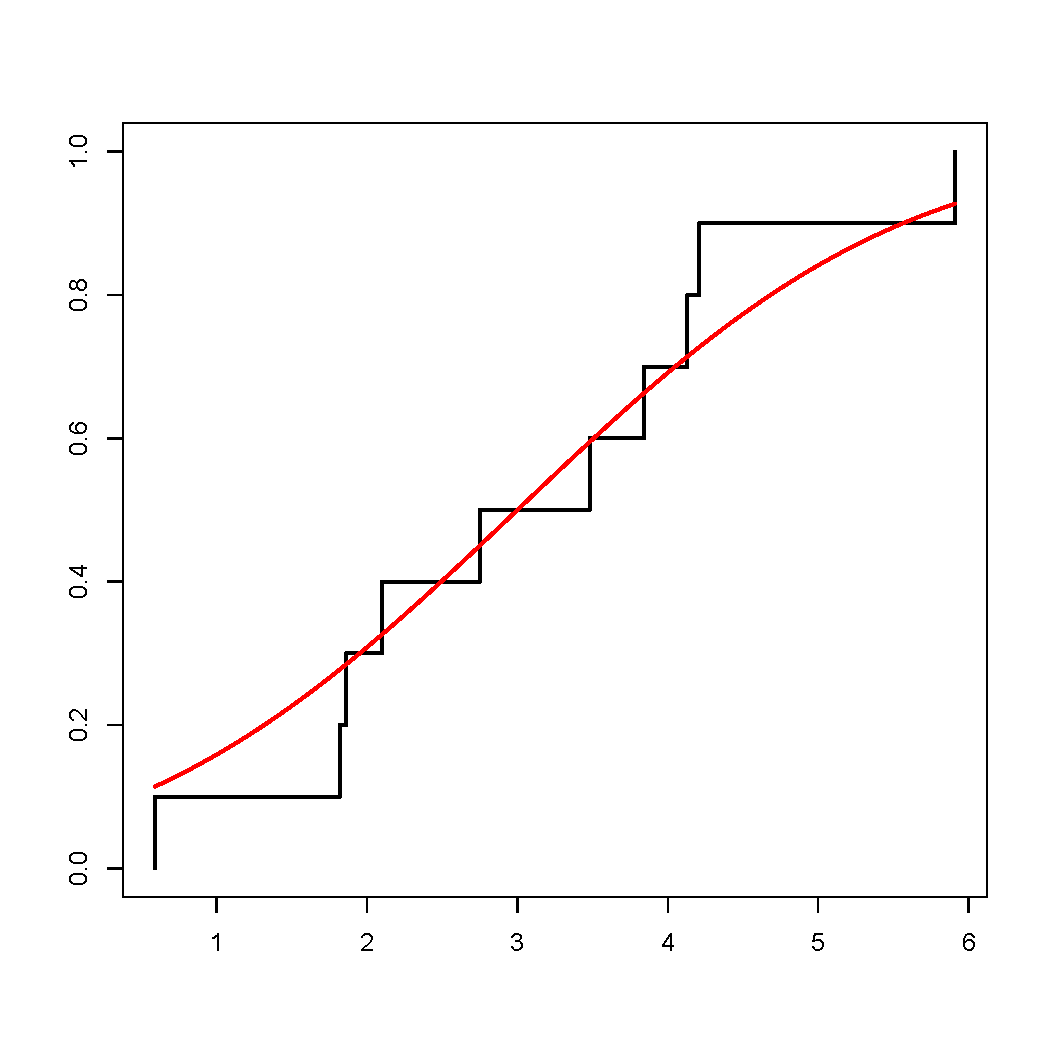
\includegraphics[width=0.7\linewidth]{KS}
\end{center}

\end{frame}



\begin{frame}
\frametitle{Test K-S}

\blue{\bf (3)} Calculam $\sup\{|F_n(x)-F_X(x)|\mid x\in \RR\}$. Com que $F_X$ és creixent, aquest suprem s'assoleix al voltant de qualque escaló.
\vspace*{-3ex}

\begin{center}
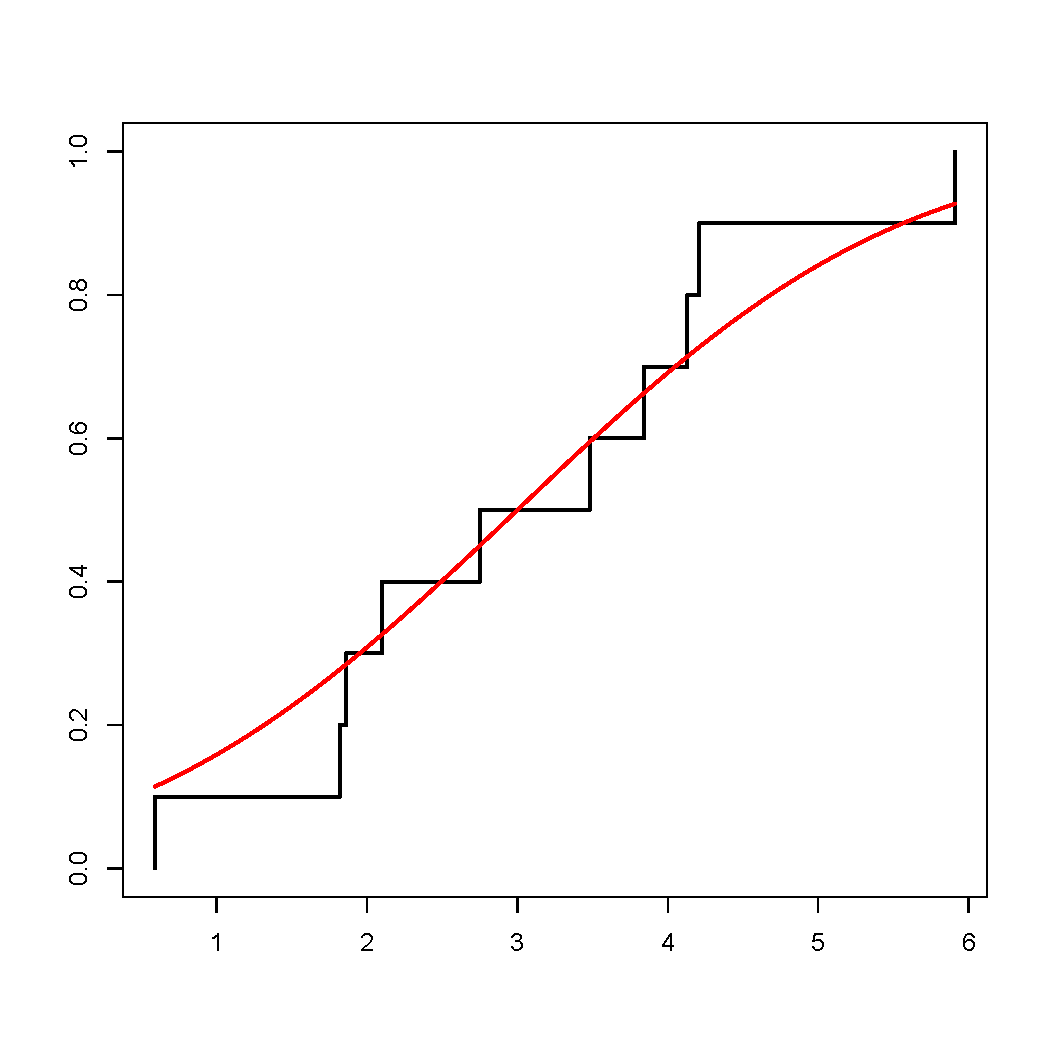
\includegraphics[width=0.7\linewidth]{KS}
\end{center}

\end{frame}

\begin{frame}
\frametitle{Test K-S}

\blue{\bf (3)} Per fer-ho, calculam, per a cada $x_{(i)}$, la \emph{discrepància}
$$
\begin{array}{rl}
D_n(x_{(i)})& \hspace*{-1.5ex} =\mbox{màx}\big\{| F_X(x_{(i)})-F_{n}(x_{(i)}^{-})|, |F_{X}(x_{(i)})-F_n(x_{(i)})|\big\}\\[1ex]
& \hspace*{-1.5ex} \displaystyle=\mbox{màx}\Big\{\Big| F_X(x_{(i)})-\frac{i-1}{n}\Big|, \Big|F_{X}(x_{(i)})-\frac{i}{n}\Big|\Big\}
\end{array}$$
(recordau \blue{$F(a^{-})=\lim\limits_{t\to a^{-}} F(t)$})


\end{frame}

\begin{frame}
\frametitle{Test K-S}

\blue{\bf (3)} \ldots\ i prenem la \emph{discrepància màxima}
$$
D_n=\mbox{màx}\big\{D_n(x_{(h)})\mid h=1,\ldots, n\big\}
$$
\medskip

Aquesta discrepància màxima segueix una distribució coneguda (que no depèn de la $X$ mentre sigui contínua) que permet calcular regions de rebuig i p-valors

\end{frame}




\begin{frame}[fragile]
\frametitle{Test K-S}

\blue{\bf Exemple}: Volem decidir si els valors
$$
5.84,4.57,1.34,3.58,1.54,2.25
$$
provenen d'una distribució normal amb $\mu=3$ i $\sigma=1.5$. 
\bigskip

Volem fer el contrast
$$
\left\{
\begin{array}{l}
H_0: \mbox{ aquesta mostra prové d'una $X\sim N(3,1.5)$}\\
H_0: \mbox{ aquesta mostra no prové d'una $X\sim N(3,1.5)$}
\end{array}
\right.
$$
\end{frame}


\begin{frame}[fragile]
\frametitle{Test K-S}

Ordenam la mostra: $x_{(1)}< x_{(2)}<\cdots< x_{(n)}$
\medskip

\blue{\bf Exemple}: Ordenam $5.84,4.57,1.34,3.58,1.54,2.25$
\begin{verbatim}
> x=c(5.84,4.57,1.34,3.58,1.54,2.25)
> sort(x)
[1] 1.34 1.54 2.25 3.58 4.57 5.84
\end{verbatim}


\end{frame}


\begin{frame}
\frametitle{Test K-S}

Calculam la \emph{funció de distribució mostral} $F_{n}$
d'aquesta mostra com si cada $x_{(i)}$ tingués probabilitat $1/n$
$$
F_n(x)=\left\{\begin{array}{ll}
0 &\mbox{ si } x< x_{(1)} \\
\dfrac{k}{n}&\mbox{ si } x_{(k)}\leq x < x_{(k+1)}\\[2ex]
1 & \mbox{ si } x_{(n)} \leq x
\end{array}
\right.
$$


\blue{\bf Exemple}: Ordenats $1.34, 1.54, 2.25, 3.58, 4.57, 5.84$:
$$
F_6(x)=\left\{\begin{array}{ll}
0 &\mbox{ si } x< 1.34 \\
1/6 &\mbox{ si } 1.34\leq x <1.54\\
2/6 &\mbox{ si } 1.54\leq x <2.25\\
3/6 &\mbox{ si } 2.25\leq x <3.58\\
4/6 &\mbox{ si } 3.58\leq x <4.57\\
5/6 &\mbox{ si } 4.57\leq x <5.84\\
1 &\mbox{ si } 5.84\leq x 
\end{array}
\right.
$$

\end{frame}






\begin{frame}[fragile]
\frametitle{Test K-S}
\vspace*{-4ex}

\begin{center}
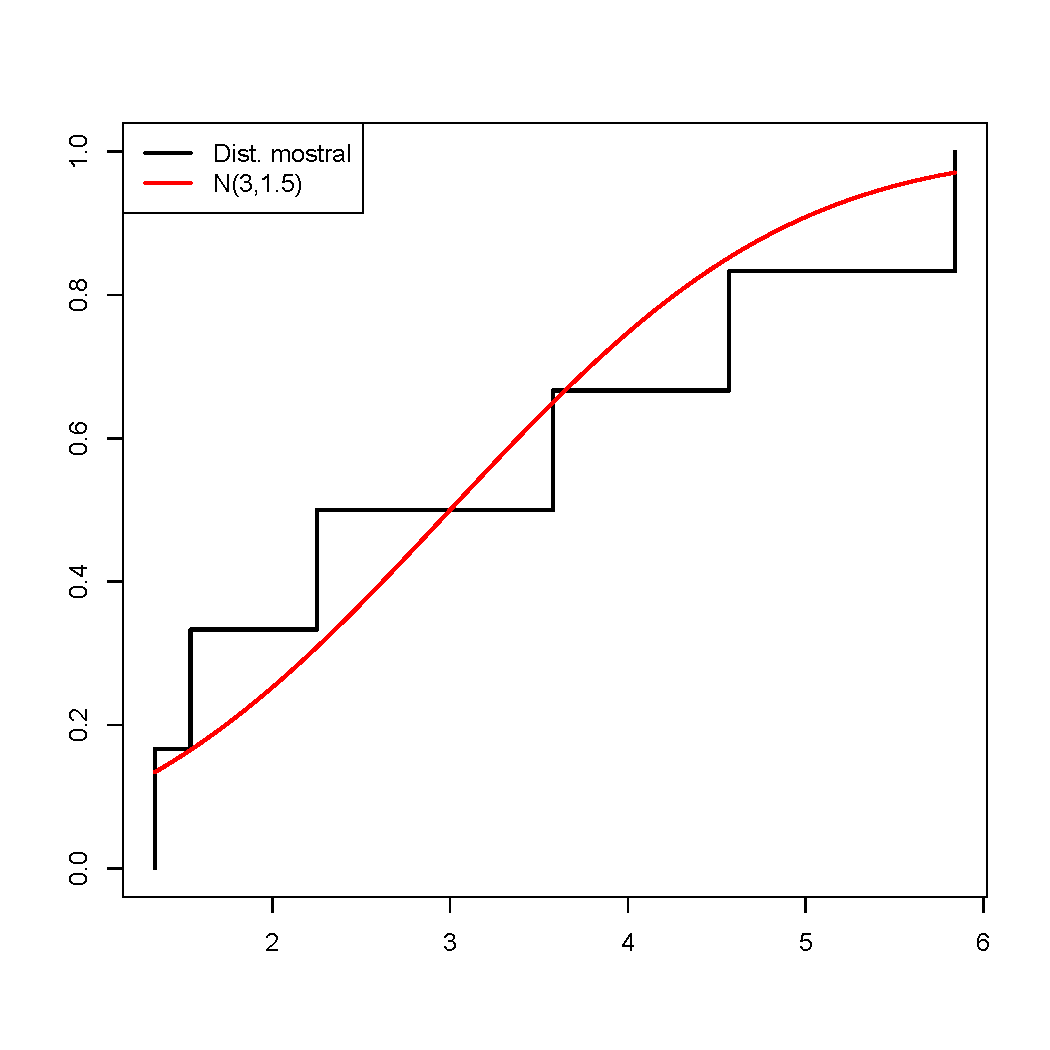
\includegraphics[width=0.8\linewidth]{KS2}
\end{center}


\end{frame}






\begin{frame}[fragile]
\frametitle{Test K-S}

Calculam la \emph{discrepància} de cada observació $x_{(i)}$
$$
D_n(x_{(i)})=\mbox{màx}\Big\{\Big| F_X(x_{(i)})-\frac{i-1}{n}\Big|, \Big|F_{X}(x_{(i)})-\frac{i}{n}\Big|\Big\}
$$

\blue{\bf Exemple}: Ordenats $1.34, 1.54, 2.25, 3.58, 4.57, 5.84$;
\begin{verbatim}
> round(pnorm(sort(x),3,1.5),3)
[1] 0.134 0.165 0.309 0.650 0.852 0.971
\end{verbatim}
\only<1>{\small $$
\begin{array}{rl}
\hspace*{-2ex} D_6(x_{(1)}) \hspace*{-1.5ex}& =\mbox{màx}\{| F_X(1.34)-0|, |F_X(1.34)-1/6|\}\\
& =\mbox{màx}\{|0.134-0|, |0.134-1/6|\}\\
& =\mbox{màx}\{ 0.134, 0.033\}=0.134\\[2ex]
\hspace*{-2ex} D_6(x_{(2)}) \hspace*{-1.5ex}& =\mbox{màx}\{| F_X(1.54)-1/6|, |F_X(1.54)-2/6|\}\\
& =\mbox{màx}\{| 0.165-1/6|, |0.165-2/6|\}\\
& =\mbox{màx}\{ 0.002, 0.168\}=0.168
\end{array}
$$
}
%
\only<2>{\small $$
\begin{array}{rl}
\hspace*{-2ex} D_6(x_{(3)}) \hspace*{-1.5ex}& =\mbox{màx}\{| F_X(2.25)-2/6|, |F_X(2.25)-3/6|\}\\
& =\mbox{màx}\{|0.309-2/6|, |0.309-3/6|\}\\
& =\mbox{màx}\{ 0.024, 0.191\}=0.191\\[2ex]
\hspace*{-2ex} D_6(x_{(4)}) \hspace*{-1.5ex}& =\mbox{màx}\{| F_X(3.58)-3/6|, |F_X(3.58)-4/6|\}\\
& =\mbox{màx}\{| 0.65-3/6|, |0.65-4/6|\}\\
& =\mbox{màx}\{ 0.15, 0.017\}=0.15
\end{array}
$$
}
%
\only<3>{\small $$
\begin{array}{rl}
\hspace*{-2ex} D_6(x_{(5)}) \hspace*{-1.5ex}& =\mbox{màx}\{| F_X(4.57)-4/6|, |F_X(4.57)-5/6|\}\\
& =\mbox{màx}\{|0.852-4/6|, |0.852-5/6|\}\\
& =\mbox{màx}\{ 0.185, 0.019\}=0.185\\[2ex]
\hspace*{-2ex} D_6(x_{(6)}) \hspace*{-1.5ex}& =\mbox{màx}\{| F_X(5.84)-5/6|, |F_X(5.84)-6/6|\}\\
& =\mbox{màx}\{| 0.971-5/6|, |0.971-1|\}\\
& =\mbox{màx}\{ 0.138, 0.029\}=0.138
\end{array}
$$
}


\end{frame}

\begin{frame}
\frametitle{Test K-S}
Definim l'estadístic \emph{$D_n$} com la discrepància més gran:
$$
D_n=\mbox{màx}\big\{D_n(x_{(h)})\mid h=1,\ldots, n\big\}
$$

\blue{\bf Exemple}: 
$$
\begin{array}{rl}
D_6& =\mbox{màx}\{0.134,0.168,0.191,0.15,0.185,0.138\}\\ &=0.191
\end{array}
$$

\end{frame}

\begin{frame}
\frametitle{Test K-S}

La \emph{regla de decisió} és rebutjar $H_0$ al nivell $\alpha$ si
$$
D_n\geq D_{n,\alpha}
$$
on $D_{n,\alpha}$ és el $\alpha$-quantil de la distribució del test K-S (teniu les taules a Campus Extens)
\medskip


\blue{\bf Exemple}: Si prenem $\alpha=0.05$, tenim que $D_{6,0.05}=0.521$.
Com que $0.191<0.521$, no podem rebutjar que la mostra provingui d'una variable $N(3,1.5)$.

\end{frame}

\begin{frame}[fragile]
\frametitle{Amb R}
\vspace*{-1ex}

Per realitzar un test K-S amb R, tenim la instrucció
\begin{center}
\texttt{ks.test(x,"distribució",paràmetres)}
\end{center} 
on \texttt{x} és el vector que analitzam, la \texttt{distribució} és la distribució que contrastam, i els \texttt{paràmetres} són els de la distribució.
\medskip


\blue{\bf Exemple}: 
\begin{verbatim}
> x=c(5.84,4.57,1.34,3.58,1.54,2.25)
> ks.test(x,"pnorm",3,1.5)
      One-sample Kolmogorov-Smirnov test
data:  x 
D = 0.1915, p-value = 0.95
alternative hypothesis: two-sided
\end{verbatim}
Dóna el valor de l'estadístic, i un p-valor amb el significat usual


\end{frame}

\begin{frame}
\frametitle{Test K-S-Lilliefors}

Quan es fa el test K-S per contrastar si una mostra prové d'una distribució \emph{normal amb $\mu$ i $\sigma$ desconegudes}, es recomana
\begin{itemize}
\item Estimar els paràmetres de la normal a partir de la mostra
\medskip

\item Calcular l'estadístic del test K-S amb aquests paràmetres
\medskip

\item Emprar  a la decisió els $\alpha$-quantils $D'_{n,\alpha}$ de la distribució del \emph{test K-S-Lilliefors} (teniu la taules a Campus Extens)
\end{itemize}

\end{frame}

\begin{frame}[fragile]
\frametitle{Test K-S-Lilliefors}


Amb R, és la funció \texttt{lillie.test} del paquet \texttt{nortest}
\medskip

\blue{\bf Exemple}: 
\begin{verbatim}
> install.packages("nortest",dep=TRUE)
...
> library(nortest)
> x=c(5.84,4.57,1.34,3.58,1.54,2.25)
> lillie.test(x)
     Lilliefors (Kolmogorov-Smirnov) normality 
     test
data:  x 
D = 0.1991, p-value = 0.6425
\end{verbatim}

\end{frame}



    
%%%%%%%%%%%%%%%%%%%%

\section{Independència}
\subsection{Test $\chi^2$}

\begin{frame}
\frametitle{Test $\chi^2$ d'independència en taules de contingència}

Tenim una taula de contingència que ens dóna les freqüències absolutes conjuntes de dues característiques  $X$ i $Y$ d'una població. Volem contrastar si aquestes dues característiques són variables aleatòries
independents  o no.

\end{frame}

\begin{frame}
\frametitle{Exemple 5}

En un estudi d'una vacuna d'hepatitis hi participen $1083$ voluntaris. D'aquests, es trien aleatòriament $549$ i són vacunats. Els altres, $534$, no són vacunats. Després d'un cert temps, s'observa que $70$ dels $534$ no vacunats han agafat l'hepatitis, mentre que només $11$ dels $549$ vacunats l'han agafada.
\begin{center}
 \begin{tabular}{c|cc}
\hline &\multicolumn{2}{c}{Vacunat?}\\\hline 
Emmalaltí?& Sí &No \\\hline
Sí &11& 70 \\
No& 538 &464\\\hline
 \end{tabular}
\end{center}
És el fet de contreure hepatitis
independent d'haver estat vacunat contra la malaltia?

\end{frame}

\begin{frame}
\frametitle{Exemple 5}

\begin{center}
 \begin{tabular}{c|cc}
\hline &\multicolumn{2}{c}{Vacunat?}\\\hline 
Emmalaltí?& Sí &No \\\hline
Sí &11& 70 \\
No& 538 &464\\\hline
 \end{tabular}
\end{center}
És el fet de contreure hepatitis
independent d'haver estat vacunat contra la malaltia?
\medskip

En aquest cas $2\times 2$ és un contrast de proporcions per a dues mostres independents:
$$
\left\{
\begin{array}{l}
H_0: p_{\,\mathrm{Vacunats}}=p_{\,\mathrm{No\hspace*{0.3ex} vacunats}}\\
H_1: p_{\,\mathrm{Vacunats}}\neq p_{\,\mathrm{No\hspace*{0.3ex} vacunats}}
\end{array}
\right.
$$
Però en general \ldots




\end{frame}


\begin{frame}
\frametitle{Test $\chi^2$ d'independència}
\vspace*{-2ex}

Considerem dues característiques $X$ i $Y$ d'una població que poden prendre els
valors $X_{1},\ldots,X_{I}$ i $Y_{1},\ldots,Y_{J}$. Donam en una taula les freqüències absolutes
de cada combinació de valors $(X_a,Y_b)$ en una mostra aleatòria de mida $n$
\begin{table}
\centering
\begin{tabular}{|c|cccccc|c|}
\hline $X\mbox{\textbackslash} Y$ & $Y_1$ & $Y_2$ & $\ldots$ & $Y_j$ & $\ldots$
& $Y_J$ & $n_{i \bullet}$ \\
\hline $X_1$ & $n_{11}$ & $n_{12}$ & $\ldots$ & $n_{1j}$ & $\ldots$ & $n_{1J}$ &
$n_{1
\bullet}$ \\ $X_2$ & $n_{21}$ & $n_{22}$ & $\ldots$ & $n_{2j}$ & $\ldots$ &
$n_{2J}$ &
$n_{2 \bullet}$ \\ $\vdots$ & $\vdots$ & $\vdots$ & $\vdots$ & $\vdots$ &
$\vdots$ &
$\vdots$ & $\vdots$ \\ $X_i$ & $n_{i1}$ & $n_{i2}$ & $\ldots$ & $n_{ij}$ &
$\ldots$ &
$n_{iJ}$ & $n_{i \bullet}$ \\ $\vdots$ & $\vdots$ & $\vdots$ & $\vdots$ &
$\vdots$ &
$\vdots$ & $\vdots$ & $\vdots$ \\ $X_I$ & $n_{I1}$ & $n_{I2}$ & $\ldots$ &
$n_{Ij}$ &
$\ldots$ & $n_{IJ}$ & $n_{I \bullet}$ \\ \hline $n_{\bullet j}$ & $n_{\bullet
1}$ &
$n_{\bullet 2}$ & $\ldots$ & $n_{\bullet j}$ & $\ldots$ & $n_{\bullet J}$ &
$n$ \\ \hline
\end{tabular}
\end{table}
\end{frame}



\begin{frame}
\frametitle{Exemple 5}

\begin{center}
 \begin{tabular}{|c|cc|c|}
 \hline
E\textbackslash V& $V_1$ & $V_2$ & $n_{i\bullet}$\\\hline
$E_1$ &11& 70  & 81\\
$E_2$ & 538 &464& 1002 \\\hline
$n_{\bullet j} $& 549 & 534 & 1083\\
\hline
 \end{tabular}
\end{center}

\end{frame}



\begin{frame}
\frametitle{Test $\chi^2$ d'independència}
$$
\left\{
\begin{array}{ll}
H_0: \mbox{ Les variables  $X$  i  $Y$  són independents}\\
H_1: \mbox{ Les variables  $X$  i  $Y$  no són independents}
\end{array}
\right.
$$

Si diem 
$$
\begin{array}{c}
p_{ij}=P(X=X_i, Y=Y_j)\\
p_i=P(X=X_i)\qquad
p_{j}=P(Y=Y_j)\\
\end{array}
$$
 el test d'independència equival a contrastar
$$
\left\{
\begin{array}{ll}
H_0: p_{ij}=p_i \cdot p_j \mbox{ per a tots } 1\leq i \leq I,\ 1\leq j\leq J \\
H_1: \mbox{no totes aquestes igualtats són veritat}
\end{array}
\right.
$$
\end{frame}


\begin{frame}
\frametitle{Test $\chi^2$ d'independència}
Emprarem l'estadístic 
$$
X^2=\sum\limits_{i=1}^I\sum\limits_{j=1}^J \frac{ \left( n_{ij}- \frac{n_{i\bullet}\cdot n_{\bullet j} }{n}\right)^2 } {\frac{n_{i\bullet} \cdot n_{\bullet j}}{n}}
$$
que compara cada \emph{freqüència observada} $n_{ij}$ amb la \emph{freqüència esperada}  si les variables fossin independents
$$
\dfrac{n_{i\bullet}}{n}\cdot \dfrac{n_{\bullet j}}{n}\cdot n=\dfrac{n_{i\bullet}\cdot n_{\bullet j}}{n}
$$ 

\medskip

Si $n$ és gran i cada freqüència esperada $\frac{n_{i\bullet}\cdot n_{\bullet j}}{n}$ és $\geq 5$, 
aquest estadístic segueix aproximadament una llei $\chi^2$ amb
$(I-1) \cdot (J -1)$ graus de llibertat
\end{frame}


\begin{frame}
\frametitle{Test $\chi^2$ d'independència}
Com sempre, si $\chi_0$ és el valor que pren l'estadístic de contrast, el \emph{p-valor} del contrast és
$$
P(\chi_{(I-1) \cdot (J -1)}^2\geq \chi_0),
$$
amb el significat usual
\end{frame}



\begin{frame}
\frametitle{Exemple 5}

\begin{center}
 \begin{tabular}{|c|cc|c|}
 \hline
E\textbackslash V& $V_1$ & $V_2$ & $n_{i\bullet}$\\\hline
$E_1$ &11& 70  & 81\\
$E_2$ & 538 &464& 1002 \\\hline
$n_{\bullet j} $& 549 & 534 & 1083\\
\hline
 \end{tabular}
\end{center}
Freqüències esperades
$$
\begin{array}{ll}
\displaystyle \frac{n_{1\bullet}\cdot n_{\bullet 1} }{n}=\frac{81\cdot 549}{1083}=41.06\\[2ex]
\displaystyle  \frac{n_{1\bullet}\cdot n_{\bullet 2} }{n}=\frac{81\cdot 534}{1083}=39.94\\[2ex]
\displaystyle  \frac{n_{2\bullet}\cdot n_{\bullet 1} }{n}=\frac{1002\cdot 549}{1083}=507.94\\[2ex]
\displaystyle  \frac{n_{2\bullet}\cdot n_{\bullet 2} }{n}=\frac{1002\cdot 534}{1083}=494.06
 \end{array}
 $$
\end{frame}



\begin{frame}
\frametitle{Exemple 5}
Estadístic:
$$
\begin{array}{rl}
\chi_0=& \displaystyle \frac{(11-41.06)^2}{41.06}
+ \frac{(70-39.94)^2}{39.94}\\[2ex]
& +\displaystyle \frac{(538-507.94)^2}{507.94}
+ \frac{(464-494.06)^2}{494.06}\\[2ex]
& = 48.24
\end{array}
$$
p-valor:
$$
P(\chi_1^2\geq 48.24)<0.05
$$
Per tant podem rebutjar la hipòtesi nu\l.la: vacunar-se i emmalaltir no són independents
\end{frame}






\begin{frame}
\frametitle{Exemple 6}
Un investigador vol saber si el nombre de cries per lloba és independent de la zona on visqui
\medskip

Considera 3 zones ($X$): $X_1=$``Nord'', $X_2=$``Centre'' i  $X_3=$``Sud''
\medskip

Classifica els nombres de cries ($Y$) en
$Y_1=$`` Dos o menys'', $Y_2=$`` Entre tres i cinc'',  $Y_3=$``Entre sis i vuit'' i  $Y_4=$``Nou o
més''
\end{frame}






\begin{frame}
\frametitle{Exemple 6}

Pren una mostra de 200 llobes i obté la taula següent:
\begin{center}
\begin{tabular}{|c|cccc|c|}
\hline
$X$\textbackslash $Y$ & $Y_1$ & $Y_2$ & $Y_3$ & $Y_4$ & $n_{i\bullet}$\\ \hline
$X_1$ & 5   & 8   & 15  & 22   & 50 \\
$X_2$ & 20 &26  &46   & 8  & 100\\
$X_3$ & 15  & 10  & 15   & 10   & 50 \\
\hline
$n_{\bullet j}$ & 40 & 44 & 76 & 40 & 200 \\ \hline
\end{tabular}
\end{center}

Les freqüències esperades si les variables són independents són
\begin{center}
\begin{tabular}{|c|cccc|c|}
\hline
$X$\textbackslash $Y$ & $Y_1$ & $Y_2$ & $Y_3$ & $Y_4$ & $n_{i\bullet}$\\ \hline
$X_1$ &  10 &  11 &  19 &  10 & 50 \\
$X_2$ &  20 & 22 & 38 &  20 & 100\\
$X_3$ &  10 &  11 &  19 &  10 & 50 \\
\hline
$n_{\bullet j}$ & 40 & 44 & 76 & 40 & 200 \\ \hline
\end{tabular}
\end{center}

\end{frame}


\begin{frame}
\frametitle{Exemple 6}
Volem fer el contrast
$$
\left\{
\begin{array}{ll}
H_0: \mbox{ El nombre de cries per lloba és independent}\\
\qquad\qquad\mbox{ de la zona}\\[1ex]
H_1: \mbox{ El nombre de cries per lloba no és independent}\\
\qquad\qquad\mbox{ de la zona}\\

\end{array}
\right.
$$
Empram l'estadístic de contrast
$$
X^2=\sum_{i=1}^3\sum_{j=1}^4 \frac{(\mbox{freq.obs}_{ij}-\mbox{freq.esp}_{ij})^2}{\mbox{freq.esp}_{ij}}
$$
$X^2$ segueix una llei $\chi^2$ amb $(3-1)\cdot(4-1)=6$ graus de llibertat.
\end{frame}
\begin{frame}
\frametitle{Exemple 6}

Calculam el valor de l'estadístic
$$
\chi_0=\ldots=31.6
$$
Calculam el p-valor
$$
P(\chi^2_6\geq 31.6)<0.05
$$
Per tant rebutjam la hipòtesi nu\l.la, i concloem que el nombre de cries per lloba és dependent de la zona on visqui.
\end{frame}



\begin{frame}[fragile]
\frametitle{Exemple 6}
Podem emprar la funció \texttt{chisq.test}, però hi hem d'entrar la taula en format \texttt{table}:
{\small \begin{verbatim}
> dades = as.table(matrix(c(5,8,15,22,20,26,46,
 8,15,10,15,10),nrow=4,byrow=TRUE))
> dades
   A  B  C  D
A  5  8 15 22
B 20 26 46  8
C 15 10 15 10
> chisq.test(dades)
     Pearson's Chi-squared test
data: dades
X-squared = 31.6048, df = 6, p-value =1.942e-05
\end{verbatim}
}

El $p$-valor és molt petit, rebutjam la hipòtesi nu\l.la
\end{frame}

\subsection{Homogeneïtat}


\begin{frame}
\frametitle{Contrast d'homogeneïtat}


Tenim una taula de contingència que ens dóna les freqüències absolutes conjuntes de dues característiques $X$ i $Y$ d'una població. Volem contrastar si, per a cada valor de $X$, les proporcions dels valors de $Y$ són les mateixes o no.
\medskip

\blue{\bf Exemple:} En el nostre exemple de la vacuna
\begin{center}
 \begin{tabular}{c|cc}
\hline &\multicolumn{2}{c}{Vacunat?}\\\hline 
Emmalaltí?& Sí &No \\\hline
Sí &11& 70 \\
No& 538 &464\\\hline
 \end{tabular}
\end{center}
volem determinar si la proporció de malalts és la mateixa entre els vacunats que entre els que no estan vacunats
\end{frame}


\begin{frame}
\frametitle{Contrast d'homogeneïtat}



És exactament el mateix test que el d'independència (si les variables són independents, les proporcions no variaran segons la filera o segons la columna)
\medskip

Però el disseny de l'experiment sol ser diferent: usualment, l'experimentador tria \textsl{a priori} el nombre d'unitats experimentals per a cada valor $X_i$ de $X$ (és el que hem fet a l'exemple de les vacunes, però no el que hem fet a l'exemple dels llops)
\end{frame}

\end{document}